% Auto-generated graphical tensor slide snippets
\newcommand{\PDa}{%
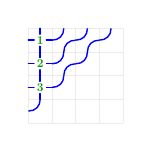
\begin{tikzpicture}[baseline=(current bounding box.center),scale=0.3]
  \draw[lightgray, very thin, opacity=0.3] (0,0) -- (4,0);
  \draw[lightgray, very thin, opacity=0.3] (0,0) -- (0,4);
  \draw[lightgray, very thin, opacity=0.3] (0,1) -- (4,1);
  \draw[lightgray, very thin, opacity=0.3] (1,0) -- (1,4);
  \draw[lightgray, very thin, opacity=0.3] (0,2) -- (4,2);
  \draw[lightgray, very thin, opacity=0.3] (2,0) -- (2,4);
  \draw[lightgray, very thin, opacity=0.3] (0,3) -- (4,3);
  \draw[lightgray, very thin, opacity=0.3] (3,0) -- (3,4);
  \draw[lightgray, very thin, opacity=0.3] (0,4) -- (4,4);
  \draw[lightgray, very thin, opacity=0.3] (4,0) -- (4,4);
  \draw[blue, line width=0.5pt, line cap=round] (0,3.5) -- (1,3.5);
  \draw[blue, line width=0.5pt, line cap=round] (0.5,3) -- (0.5,4);
  \draw[blue, line width=0.5pt] (1,3.5) .. controls (1.3,3.5) and (1.5,3.7) .. (1.5,4);
  \draw[blue, line width=0.5pt] (1.5,3) .. controls (1.5,3.3) and (1.7,3.5) .. (2,3.5);
  \draw[blue, line width=0.5pt] (2,3.5) .. controls (2.3,3.5) and (2.5,3.7) .. (2.5,4);
  \draw[blue, line width=0.5pt] (2.5,3) .. controls (2.5,3.3) and (2.7,3.5) .. (3,3.5);
  \draw[blue, line width=0.5pt] (3,3.5) .. controls (3.3,3.5) and (3.5,3.7) .. (3.5,4);
  \draw[blue, line width=0.5pt, line cap=round] (0,2.5) -- (1,2.5);
  \draw[blue, line width=0.5pt, line cap=round] (0.5,2) -- (0.5,3);
  \draw[blue, line width=0.5pt] (1,2.5) .. controls (1.3,2.5) and (1.5,2.7) .. (1.5,3);
  \draw[blue, line width=0.5pt] (1.5,2) .. controls (1.5,2.3) and (1.7,2.5) .. (2,2.5);
  \draw[blue, line width=0.5pt] (2,2.5) .. controls (2.3,2.5) and (2.5,2.7) .. (2.5,3);
  \draw[blue, line width=0.5pt, line cap=round] (0,1.5) -- (1,1.5);
  \draw[blue, line width=0.5pt, line cap=round] (0.5,1) -- (0.5,2);
  \draw[blue, line width=0.5pt] (1,1.5) .. controls (1.3,1.5) and (1.5,1.7) .. (1.5,2);
  \draw[blue, line width=0.5pt] (0,0.5) .. controls (0.3,0.5) and (0.5,0.7) .. (0.5,1);
  \node[font=\Large\bfseries, text=green!60!black, fill=white, inner sep=0.5pt, circle, transform shape] at (0.5,1.5) {3};
  \node[font=\Large\bfseries, text=green!60!black, fill=white, inner sep=0.5pt, circle, transform shape] at (0.5,3.5) {1};
  \node[font=\Large\bfseries, text=green!60!black, fill=white, inner sep=0.5pt, circle, transform shape] at (0.5,2.5) {2};
\end{tikzpicture}
}
\newcommand{\PDb}{%
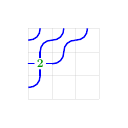
\begin{tikzpicture}[baseline=(current bounding box.center),scale=0.3]
  \draw[lightgray, very thin, opacity=0.3] (0,0) -- (3,0);
  \draw[lightgray, very thin, opacity=0.3] (0,0) -- (0,3);
  \draw[lightgray, very thin, opacity=0.3] (0,1) -- (3,1);
  \draw[lightgray, very thin, opacity=0.3] (1,0) -- (1,3);
  \draw[lightgray, very thin, opacity=0.3] (0,2) -- (3,2);
  \draw[lightgray, very thin, opacity=0.3] (2,0) -- (2,3);
  \draw[lightgray, very thin, opacity=0.3] (0,3) -- (3,3);
  \draw[lightgray, very thin, opacity=0.3] (3,0) -- (3,3);
  \draw[blue, line width=0.5pt] (0,2.5) .. controls (0.3,2.5) and (0.5,2.7) .. (0.5,3);
  \draw[blue, line width=0.5pt] (0.5,2) .. controls (0.5,2.3) and (0.7,2.5) .. (1,2.5);
  \draw[blue, line width=0.5pt] (1,2.5) .. controls (1.3,2.5) and (1.5,2.7) .. (1.5,3);
  \draw[blue, line width=0.5pt] (1.5,2) .. controls (1.5,2.3) and (1.7,2.5) .. (2,2.5);
  \draw[blue, line width=0.5pt] (2,2.5) .. controls (2.3,2.5) and (2.5,2.7) .. (2.5,3);
  \draw[blue, line width=0.5pt, line cap=round] (0,1.5) -- (1,1.5);
  \draw[blue, line width=0.5pt, line cap=round] (0.5,1) -- (0.5,2);
  \draw[blue, line width=0.5pt] (1,1.5) .. controls (1.3,1.5) and (1.5,1.7) .. (1.5,2);
  \draw[blue, line width=0.5pt] (0,0.5) .. controls (0.3,0.5) and (0.5,0.7) .. (0.5,1);
  \node[font=\Large\bfseries, text=green!60!black, fill=white, inner sep=0.5pt, circle, transform shape] at (0.5,1.5) {2};
\end{tikzpicture}
}
\newcommand{\PDc}{%
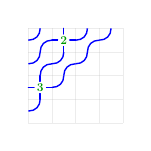
\begin{tikzpicture}[baseline=(current bounding box.center),scale=0.3]
  \draw[lightgray, very thin, opacity=0.3] (0,0) -- (4,0);
  \draw[lightgray, very thin, opacity=0.3] (0,0) -- (0,4);
  \draw[lightgray, very thin, opacity=0.3] (0,1) -- (4,1);
  \draw[lightgray, very thin, opacity=0.3] (1,0) -- (1,4);
  \draw[lightgray, very thin, opacity=0.3] (0,2) -- (4,2);
  \draw[lightgray, very thin, opacity=0.3] (2,0) -- (2,4);
  \draw[lightgray, very thin, opacity=0.3] (0,3) -- (4,3);
  \draw[lightgray, very thin, opacity=0.3] (3,0) -- (3,4);
  \draw[lightgray, very thin, opacity=0.3] (0,4) -- (4,4);
  \draw[lightgray, very thin, opacity=0.3] (4,0) -- (4,4);
  \draw[blue, line width=0.5pt] (0,3.5) .. controls (0.3,3.5) and (0.5,3.7) .. (0.5,4);
  \draw[blue, line width=0.5pt] (0.5,3) .. controls (0.5,3.3) and (0.7,3.5) .. (1,3.5);
  \draw[blue, line width=0.5pt, line cap=round] (1,3.5) -- (2,3.5);
  \draw[blue, line width=0.5pt, line cap=round] (1.5,3) -- (1.5,4);
  \draw[blue, line width=0.5pt] (2,3.5) .. controls (2.3,3.5) and (2.5,3.7) .. (2.5,4);
  \draw[blue, line width=0.5pt] (2.5,3) .. controls (2.5,3.3) and (2.7,3.5) .. (3,3.5);
  \draw[blue, line width=0.5pt] (3,3.5) .. controls (3.3,3.5) and (3.5,3.7) .. (3.5,4);
  \draw[blue, line width=0.5pt] (0,2.5) .. controls (0.3,2.5) and (0.5,2.7) .. (0.5,3);
  \draw[blue, line width=0.5pt] (0.5,2) .. controls (0.5,2.3) and (0.7,2.5) .. (1,2.5);
  \draw[blue, line width=0.5pt] (1,2.5) .. controls (1.3,2.5) and (1.5,2.7) .. (1.5,3);
  \draw[blue, line width=0.5pt] (1.5,2) .. controls (1.5,2.3) and (1.7,2.5) .. (2,2.5);
  \draw[blue, line width=0.5pt] (2,2.5) .. controls (2.3,2.5) and (2.5,2.7) .. (2.5,3);
  \draw[blue, line width=0.5pt, line cap=round] (0,1.5) -- (1,1.5);
  \draw[blue, line width=0.5pt, line cap=round] (0.5,1) -- (0.5,2);
  \draw[blue, line width=0.5pt] (1,1.5) .. controls (1.3,1.5) and (1.5,1.7) .. (1.5,2);
  \draw[blue, line width=0.5pt] (0,0.5) .. controls (0.3,0.5) and (0.5,0.7) .. (0.5,1);
  \node[font=\Large\bfseries, text=green!60!black, fill=white, inner sep=0.5pt, circle, transform shape] at (0.5,1.5) {3};
  \node[font=\Large\bfseries, text=green!60!black, fill=white, inner sep=0.5pt, circle, transform shape] at (1.5,3.5) {2};
\end{tikzpicture}
}
\newcommand{\PDd}{%
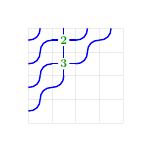
\begin{tikzpicture}[baseline=(current bounding box.center),scale=0.3]
  \draw[lightgray, very thin, opacity=0.3] (0,0) -- (4,0);
  \draw[lightgray, very thin, opacity=0.3] (0,0) -- (0,4);
  \draw[lightgray, very thin, opacity=0.3] (0,1) -- (4,1);
  \draw[lightgray, very thin, opacity=0.3] (1,0) -- (1,4);
  \draw[lightgray, very thin, opacity=0.3] (0,2) -- (4,2);
  \draw[lightgray, very thin, opacity=0.3] (2,0) -- (2,4);
  \draw[lightgray, very thin, opacity=0.3] (0,3) -- (4,3);
  \draw[lightgray, very thin, opacity=0.3] (3,0) -- (3,4);
  \draw[lightgray, very thin, opacity=0.3] (0,4) -- (4,4);
  \draw[lightgray, very thin, opacity=0.3] (4,0) -- (4,4);
  \draw[blue, line width=0.5pt] (0,3.5) .. controls (0.3,3.5) and (0.5,3.7) .. (0.5,4);
  \draw[blue, line width=0.5pt] (0.5,3) .. controls (0.5,3.3) and (0.7,3.5) .. (1,3.5);
  \draw[blue, line width=0.5pt, line cap=round] (1,3.5) -- (2,3.5);
  \draw[blue, line width=0.5pt, line cap=round] (1.5,3) -- (1.5,4);
  \draw[blue, line width=0.5pt] (2,3.5) .. controls (2.3,3.5) and (2.5,3.7) .. (2.5,4);
  \draw[blue, line width=0.5pt] (2.5,3) .. controls (2.5,3.3) and (2.7,3.5) .. (3,3.5);
  \draw[blue, line width=0.5pt] (3,3.5) .. controls (3.3,3.5) and (3.5,3.7) .. (3.5,4);
  \draw[blue, line width=0.5pt] (0,2.5) .. controls (0.3,2.5) and (0.5,2.7) .. (0.5,3);
  \draw[blue, line width=0.5pt] (0.5,2) .. controls (0.5,2.3) and (0.7,2.5) .. (1,2.5);
  \draw[blue, line width=0.5pt, line cap=round] (1,2.5) -- (2,2.5);
  \draw[blue, line width=0.5pt, line cap=round] (1.5,2) -- (1.5,3);
  \draw[blue, line width=0.5pt] (2,2.5) .. controls (2.3,2.5) and (2.5,2.7) .. (2.5,3);
  \draw[blue, line width=0.5pt] (0,1.5) .. controls (0.3,1.5) and (0.5,1.7) .. (0.5,2);
  \draw[blue, line width=0.5pt] (0.5,1) .. controls (0.5,1.3) and (0.7,1.5) .. (1,1.5);
  \draw[blue, line width=0.5pt] (1,1.5) .. controls (1.3,1.5) and (1.5,1.7) .. (1.5,2);
  \draw[blue, line width=0.5pt] (0,0.5) .. controls (0.3,0.5) and (0.5,0.7) .. (0.5,1);
  \node[font=\Large\bfseries, text=green!60!black, fill=white, inner sep=0.5pt, circle, transform shape] at (1.5,3.5) {2};
  \node[font=\Large\bfseries, text=green!60!black, fill=white, inner sep=0.5pt, circle, transform shape] at (1.5,2.5) {3};
\end{tikzpicture}
}
\newcommand{\PDe}{%
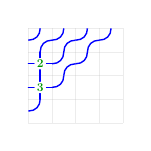
\begin{tikzpicture}[baseline=(current bounding box.center),scale=0.3]
  \draw[lightgray, very thin, opacity=0.3] (0,0) -- (4,0);
  \draw[lightgray, very thin, opacity=0.3] (0,0) -- (0,4);
  \draw[lightgray, very thin, opacity=0.3] (0,1) -- (4,1);
  \draw[lightgray, very thin, opacity=0.3] (1,0) -- (1,4);
  \draw[lightgray, very thin, opacity=0.3] (0,2) -- (4,2);
  \draw[lightgray, very thin, opacity=0.3] (2,0) -- (2,4);
  \draw[lightgray, very thin, opacity=0.3] (0,3) -- (4,3);
  \draw[lightgray, very thin, opacity=0.3] (3,0) -- (3,4);
  \draw[lightgray, very thin, opacity=0.3] (0,4) -- (4,4);
  \draw[lightgray, very thin, opacity=0.3] (4,0) -- (4,4);
  \draw[blue, line width=0.5pt] (0,3.5) .. controls (0.3,3.5) and (0.5,3.7) .. (0.5,4);
  \draw[blue, line width=0.5pt] (0.5,3) .. controls (0.5,3.3) and (0.7,3.5) .. (1,3.5);
  \draw[blue, line width=0.5pt] (1,3.5) .. controls (1.3,3.5) and (1.5,3.7) .. (1.5,4);
  \draw[blue, line width=0.5pt] (1.5,3) .. controls (1.5,3.3) and (1.7,3.5) .. (2,3.5);
  \draw[blue, line width=0.5pt] (2,3.5) .. controls (2.3,3.5) and (2.5,3.7) .. (2.5,4);
  \draw[blue, line width=0.5pt] (2.5,3) .. controls (2.5,3.3) and (2.7,3.5) .. (3,3.5);
  \draw[blue, line width=0.5pt] (3,3.5) .. controls (3.3,3.5) and (3.5,3.7) .. (3.5,4);
  \draw[blue, line width=0.5pt, line cap=round] (0,2.5) -- (1,2.5);
  \draw[blue, line width=0.5pt, line cap=round] (0.5,2) -- (0.5,3);
  \draw[blue, line width=0.5pt] (1,2.5) .. controls (1.3,2.5) and (1.5,2.7) .. (1.5,3);
  \draw[blue, line width=0.5pt] (1.5,2) .. controls (1.5,2.3) and (1.7,2.5) .. (2,2.5);
  \draw[blue, line width=0.5pt] (2,2.5) .. controls (2.3,2.5) and (2.5,2.7) .. (2.5,3);
  \draw[blue, line width=0.5pt, line cap=round] (0,1.5) -- (1,1.5);
  \draw[blue, line width=0.5pt, line cap=round] (0.5,1) -- (0.5,2);
  \draw[blue, line width=0.5pt] (1,1.5) .. controls (1.3,1.5) and (1.5,1.7) .. (1.5,2);
  \draw[blue, line width=0.5pt] (0,0.5) .. controls (0.3,0.5) and (0.5,0.7) .. (0.5,1);
  \node[font=\Large\bfseries, text=green!60!black, fill=white, inner sep=0.5pt, circle, transform shape] at (0.5,1.5) {3};
  \node[font=\Large\bfseries, text=green!60!black, fill=white, inner sep=0.5pt, circle, transform shape] at (0.5,2.5) {2};
\end{tikzpicture}
}
\newcommand{\PDf}{%
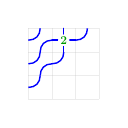
\begin{tikzpicture}[baseline=(current bounding box.center),scale=0.3]
  \draw[lightgray, very thin, opacity=0.3] (0,0) -- (3,0);
  \draw[lightgray, very thin, opacity=0.3] (0,0) -- (0,3);
  \draw[lightgray, very thin, opacity=0.3] (0,1) -- (3,1);
  \draw[lightgray, very thin, opacity=0.3] (1,0) -- (1,3);
  \draw[lightgray, very thin, opacity=0.3] (0,2) -- (3,2);
  \draw[lightgray, very thin, opacity=0.3] (2,0) -- (2,3);
  \draw[lightgray, very thin, opacity=0.3] (0,3) -- (3,3);
  \draw[lightgray, very thin, opacity=0.3] (3,0) -- (3,3);
  \draw[blue, line width=0.5pt] (0,2.5) .. controls (0.3,2.5) and (0.5,2.7) .. (0.5,3);
  \draw[blue, line width=0.5pt] (0.5,2) .. controls (0.5,2.3) and (0.7,2.5) .. (1,2.5);
  \draw[blue, line width=0.5pt, line cap=round] (1,2.5) -- (2,2.5);
  \draw[blue, line width=0.5pt, line cap=round] (1.5,2) -- (1.5,3);
  \draw[blue, line width=0.5pt] (2,2.5) .. controls (2.3,2.5) and (2.5,2.7) .. (2.5,3);
  \draw[blue, line width=0.5pt] (0,1.5) .. controls (0.3,1.5) and (0.5,1.7) .. (0.5,2);
  \draw[blue, line width=0.5pt] (0.5,1) .. controls (0.5,1.3) and (0.7,1.5) .. (1,1.5);
  \draw[blue, line width=0.5pt] (1,1.5) .. controls (1.3,1.5) and (1.5,1.7) .. (1.5,2);
  \draw[blue, line width=0.5pt] (0,0.5) .. controls (0.3,0.5) and (0.5,0.7) .. (0.5,1);
  \node[font=\Large\bfseries, text=green!60!black, fill=white, inner sep=0.5pt, circle, transform shape] at (1.5,2.5) {2};
\end{tikzpicture}
}

\begin{frame}{Caveat}
  \textbf{Caveat.} The elements $\sch_w^{(n)}$ are not usually nonnegative in the Grassmannian pipe dream basis of $\mathcal{B}_n$.
  \small
  \vspace{0.1em}
  \begin{align*}
    \sch_{1432}^{(3)} ={}& -\,\PDa +\,\PDb\otimes\PDc +\,\PDb\otimes\PDd +\,\PDb\otimes\PDe \\
    & +\,\PDf\otimes\PDc +\,\PDf\otimes\PDd +\,\PDf\otimes\PDe
  \end{align*}
  \vspace{-0.4em}
  \begin{theorem}[S, $2026+$]
  This formula is nonnegative when both $u$ and $v$ avoid $1432$, $3142$, and $4132$.
  \end{theorem}
\end{frame}